
%-------------------------------------------------------------------------------
\chapter{State Estimation for Sampled-Data Systems}\label{sec:methods}
\vspace{-1cm} \label{cap4}
%
%\begin{flushright}
%\begin{minipage}{0.7\linewidth}
%\emph{``Se quiser por � prova o car�ter de um homem, d�-lhe
%poder.''}
%\end{minipage}
%\end{flushright}
%
%\begin{flushright}
%{Abraham Lincoln}
%\end{flushright}
%
%\section{Introdu��o}\label{introducao_cap_3}
%\markright{\thesection ~~~ Modelos de Previs�o} \label{previsao}
%
%

In this chapter, the field of sensor fusion under irregular sampling is resumed to the problem of estimating the states of a system with a known process model, that is observed by aperiodically sampled measurements. We begin by describing the discrete-time representation for sampled-data systems. Then we review the adopted state estimation algorithm, that is the Kalman Filter, which is the most common approach to probabilistic data fusion. The nonlinear extension based on the unscented transform is also explored.
In Section~\ref{sec:estimation_aperiodic} we describe the particularities of the filtering algorithms for when the correct time-stamp is available to the estimator and when it is not. We end with a description of the performance criteria used for assessment of the results, designed to quantify estimation accuracy and consistency.

\section{Discrete-Time Representation of Sampled-Data Systems}\label{sec:discretization}

State estimation for nonlinear sampled-data systems can be performed using the continuous-time process model and the discrete-time observation model. The state-estimate propagation is performed using numerical integration over the time interval defined by the arrivals of two consecutive measurements. The work of \citep{Teixeira20082} compares two of those methods, the sampled-data extended Kalman Filter (SDEKF) and the sampled-data unscented Kalman Filter (SDUKF) to estimate the trajectory of a satellite.

To avoid computational complexity of the numerical integrations, discretization of the process model is widely used in state estimation applications \citep{Aguirre2005}, which motivates the use of discrete-time methods in this study. Thus the system described in Section \ref{sec:problem_form} needs to be formulated as a discrete-time model. First, we reproduce the stochastic nonlinear sampled system models as follows


\begin{align}
\dot{x}(t) &= f(x(t), u(t), w(t), t),   \label{eq:prob_process2} \\ 
y(t_k) &= g(x(t_k) ,v(t_k), t_k), \label{eq:prob_obs2}
\end{align}

\noindent
where $f\!\!: \mathbb{R}^n \times \mathbb{R}^p \times \mathbb{R}^q \times \mathbb{R^+} \rightarrow \mathbb{R}^n $ and $g\!\!: \mathbb{R}^n \times \mathbb{R}^r \times \mathbb{R^+} \rightarrow \mathbb{R}^m $ are, respectively, the process and observation models, $k \in \mathbb{N}$ is the discrete-time index, $t_k$ represents the irregular time instants, $x(t) \in \mathbb{R}^n$ the state vector,  $u(t) \in \mathbb{R}^p$ is the input vector and $w(t) \in \mathbb{R}^q$ is the process noise vector, all at continuous-time $t$, $y(t_k) \in \mathbb{R}^m$ represents the irregularly sampled measurement sequence and $v(t_k) \in \mathbb{R}^r$ the corresponding measurement noise vector. Initial condition $x_0$ is assumed to be known.

The continuous-time system dynamics defined by (\ref{eq:prob_process2}) is discretized replacing the differentiation by differencing, via numerical methods. For this study we use the fourth order Runge-Kutta method~\citep{Suli2003}, given by

\begin{align}
x(t_{k+1})&= x({t_k}) + \frac{1}{6} \left( k_1 + 2k_2 +  3k_3 + k_4\right), \label{eq:runge_kutta} \\
t_{k+1} &= t_k + h_k, \label{eq:time_interval}
\end{align}

\noindent
where $h_k \in \mathbb{R}$ is the variable step size, defined by random time intervals, and

\begin{align}
k_1 &= h_k f(t_k, \ x({t_k})), \label{eq:runge_kutta22}\\ 
k_2 &= h_k f(t_k + \frac{h_k}{2}, \ x({t_k}) + \frac{k_1}{2}), \\
k_3 &= h_k f(t_k + \frac{h_k}{2}, \ x({t_k}) + \frac{k_2}{2}), \\
k_4 &= h_k f(t_k + h_k, \ x({t_k}) + k_3), \label{eq:runge_kutta2}
\end{align}

\noindent
where $f(x(t), u(t), w(t), t)$ was reduce to $f(x(t), t)$ for simplicity, since the numerical approximation depends only on the vector state itself and the time intervals. Input $u(t)$ is considered to be constant during the time step and $w(t)$ represents unknown noise. Therefore, the discrete-time representation for the nonlinear sampled system becomes

\begin{align}
x(t_{k+1}) &= f_\textrm{d}(x(t_k), u(t_k), w(t_k), t_k),   \label{eq:prob_process3} \\ 
y(t_k) &= g(x(t_k) ,v(t_k), t_k), \label{eq:prob_obs3}
\end{align}

\noindent
where $f_\textrm{d}(\cdot)$ is given by (\ref{eq:runge_kutta})-(\ref{eq:runge_kutta2}). Note that even if the nonlinear dynamics given by (\ref{eq:prob_process2}) is time-invariant, that is if $f(\cdot)$ does not depend directly on $t$, its discrete counterpart will be time-varying if the system is irregularly sampled, since there is a time-step dependent factor $h_k$ outside $f(\cdot)$ for each $k_n$, $n=[1,2,3,4]$, in (\ref{eq:runge_kutta22})-(\ref{eq:runge_kutta2}). Discrete time instants $t_k$ are determined by random time intervals $h_k$, that is $t_{k+1} = t_k + h_k$, $\in \mathbb{R}$ as in (\ref{eq:time_interval}) and $k \in \mathbb{N}$ is the discrete-time index.

For the linear time-invariant case (LTI), dynamic model of the sampled system is given by

\begin{align}
\dot{x}(t) &= Ax(t) + Bu(t) + Gw(t),   \label{eq:prob_LTI} \\ 
y(t_k) &= Cx(t_k) + v(t_k), \label{eq:prob_LTIobs}
\end{align}

\noindent
where matrices $A \in \mathbb{R}^{n\times n}$, $B \in \mathbb{R}^{n\times p}$,  $G \in \mathbb{R}^{n\times q}$ and $C \in \mathbb{R}^{m\times n}$ are known matrices, $\rho(w(t)) = \mathcal{N}(0,Q)$ and $\rho(v(t_k)) = \mathcal{N}(0,R)$ are process and measurement noises, respectively, with covariance matrices $Q \in \mathbb{R}^{q\times q}$ and $R \in \mathbb{R}^{r \times r}$. If input $u(t)$ is digitally generated at the same rate as observations are taken, and followed by a digital-to-analog converter, then it is piecewise constant. In other words $u(t)=u(t_k)$, for $t_k \leq t < t_{k+1}$. In such cases, there is an exact solution to the discretization problem of (\ref{eq:prob_LTI}), given by \citep{Chen1999}

\begin{equation}
x(t_{k+1}) = A_\textrm{d} x(t_k) + B_\textrm{d} u(t_k) + w_\textrm{d}(t_k), \label{eq:prob_process_d}\\
\end{equation}

\noindent	
where $t_{k+1} = t_k + h_k$, $\in \mathbb{R}$ are discrete time instants as in (\ref{eq:time_interval}), separated by random time intervals $h_k \in \mathbb{R}$ and $k \in \mathbb{N}$ is the discrete-time index. The matrices from the discrete-time representation and the input noise $w_d(t_k)$ are given by

\begin{align}
A_\textrm{d} &= e^{A h_k}, \label{eq:Ad}\\
B_\textrm{d} &= \left( \int_{\tau=0}^{h_k}e^{A \tau}\delta \tau \right)B, \label{eq:Bd} \\	
w_\textrm{d}(t_k) &= \int_{\tau=0}^{h_k} e^{A(t_{k+1}-\tau)}Gdw(\tau) d\tau, \label{eq:wd}.
\end{align}

\noindent
Computation of $A_d$, given by the matrix exponential (\ref{eq:Ad}), can be solved by expansion in Taylor series

\begin{equation}
e^{A h_k} = I + h_kA+\frac{h_k^2A^2}{2!} + \ ... \ + \frac{h_k^nA^n}{n!} + \ ... \ = \sum_{i=0}^{\infty}\frac{h_k^iA^i}{i!}. \label{eq:disc_taylor}
\end{equation}

\noindent
By truncating (\ref{eq:disc_taylor}) at some point, $A_d$ can be approximated by matrix multiplications and additions. Taylor series can also be used to compute $B_d$. The integral factor of (\ref{eq:Bd}) can be expanded as

\begin{align}
\int_{\tau=0}^{h_k}e^{A \tau}\delta \tau &= \int_{\tau=0}^{h_k} \left( I + \tau A+\frac{\tau^2A^2}{2!} + \ ... \right) d\tau, \notag \\
&= h_kI + \frac{h_k^2A}{2!}+\frac{h_k^3A^2}{3!}+ \ ..., \label{eq:Bd_1}
\end{align}

\noindent
If $A$ is nonsingular, the series can be written as

\begin{align}
\int_{\tau=0}^{h_k}e^{A \tau}\delta \tau &= A^{-1} \left(Ah_kI + \frac{h_k^2A^2}{2!}+\frac{h_k^3A^3}{3!}+ \ ... \ + I - I \right), \notag \\
&=	A^{-1}\left( e^{A_k} - I\right). \label{eq:Bd_2}
\end{align}

\noindent Thus uniting (\ref{eq:Bd}) and (\ref{eq:Bd_2}), $B_d$ becomes

\begin{equation}
B_d = A^{-1} \left(A_d - I)B\right).
\end{equation}

If input noise $w(t)$ from (\ref{eq:prob_LTI}) is zero-mean white Gaussian, then $w_d(t_k)$ given by (\ref{eq:wd}) will also be zero-mean white Gaussian \citep{Jazwinski1970}, with covariance $Q_{k}$ given by 

\begin{equation}
Q_{k} = \int_{\tau=0}^{h_k} e^{A\tau}GQG^Te^{A^T\tau}d\tau, \label{eq:q_k-exact}
\end{equation}

\noindent
For state estimation purpose, we are interested in the calculation of (\ref{eq:q_k-exact}) at every time instant $t_k$, $k\in \mathbb{N}$, given that exact information about timestamp is available. Usually, for regularly sampled systems, discrete noise covariance is either modeled or tuned directly \citep{Wahlstrom2014}. However, if the system is sampled aperiodically, the dependency between covariance $Q_{k}$ and time interval $h_k$ must be taken into account. The calculation of (\ref{eq:q_k-exact}) is nontrivial and there are numerical methods available for computing the matrix exponential integral, at the expense of high computational costs \citep{Micheli2002}. In this study we simplify the problem, adopting a common practice in state estimation applications, that employs approximate discretization \citep{Axelsson2015}. Continuous-time noise is assumed to be piecewise constant in the interval $h_k$, that is $w(t)\approx w(t_k)$, for $t_k \leq t < t_{k+1}$. Then, (\ref{eq:prob_LTI}) is discretized by

\begin{equation}
x(t_{k+1}) = A_\textrm{d} x(t_k) + B_\textrm{d} u(t_k) + G_\textrm{d}w_\textrm{d}(t_k), \label{eq:prob_process_d2}\\
\end{equation}

\noindent
where $A_\textrm{d}$ and $B_\textrm{d}$ are given by (\ref{eq:Ad}) and (\ref{eq:Bd}) respectively, $G_\textrm{d}$ is calculated the same way as $B_\textrm{d}$, that is $G_\textrm{d} = \left( \int_{\tau=0}^{h_k}e^{A \tau}\delta \tau \right)G$ and $Q_{k}=h_kQ$.

Note that, once again, even for the time-invariant case, the matrices from the discrete-time system depend on time intervals, thus will be time-variant if sampling is aperiodic.

Usually, the covariance matrices $Q$ and $R$ of the noise vectors, that represent the noise level, are better expressed  by a signal-to-noise ratio (SNR) quantity, which relates more directly to how contaminated is a signal. It is basically a relation between the power level of the signal and of the noise, that is

\begin{equation}
SNR = \frac{P_{\textrm{signal}}}{P_{\textrm{noise}}},
\end{equation}

\noindent
where $P$ is the average power of a signal, which is directly proportional to its variance. Therefore it can also be expressed by

\begin{equation}
SNR = \frac{\sigma^2_{\textrm{signal}}}{\sigma^2_{\textrm{noise}}}.
\end{equation}

In Chapter~\ref{cap5} we use SNR definition to express the noise level present in signals, using the logarithmic decibel (dB) scale, given by

\begin{equation}
SNR_{\textrm{dB}} = 10 \log_{10}\frac{P_{\textrm{signal}}}{P_{\textrm{noise}}}, \label{eq:snr_db}
\end{equation}

In the next section we introduce the estimation problem and the Bayesian solution, considering the discrete-time models of state space representations. For simplicity, we replace $(t_k)$ argument for a subscript $k$, to represent discrete instants of time. 

\section{Bayesian Estimation}\label{sec:bayes_estimation}

The Bayesian approach to state estimation can be interpreted as a data fusion algorithm in which the inferred knowledge about the system's states is updated as new information arrives, using not just the new data, but also the prior information. For that, both the states and the arrived information are modeled as random variables (RV), hence its classification falls under the probabilistic fusion framework.

The goal of the estimator is to statistically and recursively infer the values of the system's states, that is the random vector $x_k \in \mathbb{R}^n$, from noisy data, that is the observation vector sequence $y_1,...,y_k \in \mathbb{R}^m$ and input vector sequence $u_1,...,u_k \in \mathbb{R}^p$. The corresponding conditional PDF, $\rho(x_k|(y_1,...,y_k))$, is called the \textit{posterior} PDF, describing the statistics of the random vector $x_k \in \mathbb{R}^n$, after the present and past experimental observations  $\rho(x_k|(y_1,...,y_k))$ have been assimilated and the process model has been taken into account. Thus we can find the estimation of $x_k$ using methods such as the \textit{maximum a posteriori} (MAP) or \textit{minimum mean square error} (MMSE), given by \citep{Bar-Shalom2001}

\begin{align}
\hat{x}_k^{MAP} &\triangleq \operatorname{arg}  \underset{x_k}{\operatorname{max}} \ \hat{\rho}(x_k|(y_1,...,y_k)), \label{eq:map} \\
\hat{x}_k^{MMSE} &\triangleq \operatorname{arg}  \underset{x_k}{\operatorname{min}} \ E[(\hat{x}_k-x_k)^T(\hat{x}_k-x_k)|(y_1,...,y_k)], \label{eq:mmse}
\end{align}

\noindent
where $\hat{x_k}$ is the estimated value of $x_k \in \mathbb{R}^n$, $\rho(x_k|(y_1,...,y_k))$ is the estimated posterior PDF of $x_k$ given the observation sequence, and $E[(\hat{x}_k-x_k)^T(\hat{x}_k-x_k)|(y_1,...,y_k)]$ is the variance of the random vector $x_k$, given the observation sequence. MAP can be interpreted as the bayesian approach to \textit{maximum likelihood} (ML) estimation, whereas MMSE is the counterpart of the \textit{least squares} (LS) estimator \citep{Bar-Shalom2001}. 

Finding the \textit{posterior} $\rho(x_k|(y_1,...,y_k))$ defines the complete state estimation problem, whereas the estimates $\hat{x_k}^{MAP} \in \mathbb{R}^n$ and $\hat{x_k}^{MMSE} \in \mathbb{R}^n$ are the optimal state estimates, under their optimality criteria. A recursive Bayesian solution to the state estimation problem, that is finding the \textit{posterior} PDF, considering that the system evolves according a Markov process is presented in Proposition~\ref{prop:bayes_solution}. But first, we need to define two lemmas.

\begin{lema}\label{lemma:markov} For a Markov system with initial state $x_0 \sim \rho(x_0)$, the transition PDF of the future state $x_{k+1}$ given the present state $x_k$ is independent of past states, that is

\begin{equation}\label{eq:lemma_transition}
\rho(x_{k+1} | (x_0,...,x_k)) = \rho(x_{k+1}|x_k),
\end{equation}

\noindent
and observation vector $y_k$ is independent of past observations and past states, given the present state $x_k$, that is

\begin{equation}\label{eq:lemma_likelihood}
\rho(y_k|(x_0,...,x_k,y_0,...,y_{k-1}) = \rho(y_k|x_k).
\end{equation}
\end{lema}

\begin{lema} \label{lemma:chapman}For a Markov system, we can find the transition PDF from step $n$ to step $s$ as a function of the transition densities between them and an intermediate step $r$, as long as $n>r>s$, by the Chapman-Kolmogorov equation~\citep{Papoulis1984}

\begin{equation}
\rho(x_n|x_s) = \int_{-\infty}^{\infty}\rho(x_n|x_r)\rho(x_r|x_s)dx_r.
\end{equation}
\end{lema}
\vspace{0.2cm}

Note that the systems described in Section~\ref{sec:discretization} are Markovian, since the transition or process models given by (\ref{eq:prob_process3}) and (\ref{eq:prob_LTIobs}) and the observation models given by (\ref{eq:prob_obs3}) and (\ref{eq:prob_LTIobs}) follow the conditions (\ref{eq:lemma_transition}) and (\ref{eq:lemma_likelihood}), respectively.

\begin{propo}\label{prop:bayes_solution} The posterior PDF of system states $x_k \in \mathbb{R}^n$ conditioned on the observation vector sequence $y_1,...,y_k \in \mathbb{R}^m$ is recursively given by

\begin{align}
\rho(x_{k}|(y_1,...,y_{k-1})) &= \int_{\mathbb{R}^n}\rho(x_k|x_{k-1}) \rho(x_{k-1}|y_1,...,y_{k-1})dx_{k-1} \label{eq:prop_xk1}, 
\\ \notag \\
\rho(x_k|(y_1,...,y_k)) &= \frac{\rho(y_k|x_k) \rho(x_k | (y_1,...,y_{k-1}))}{\rho(y_k|(y_1,...,y_{k-1}))}   \label{eq:prop_xk}
\end{align}
	

\noindent
where $k \in \mathbb{N}$, $\rho(y_k|x_k)$ is the \textit{likelihood PDF}, $\rho(x_k|(y_1,...,y_{k-1})$ is the \textit{prior PDF}, defined before the latest measurement, $\rho(x_{k}|x_{k-1})$ is the \textit{transition PDF} that models the evolution of $x_k$ and $\rho(y_k|(y_1,...,y_{k-1}))$ is the \textit{evidence}, also referred to as normalizing factor, or marginalization.

\end{propo}

\begin{proof}

The posterior PDF can be computed by the \textit{Bayes' rule}~\citep{Stone2013}

\begin{equation}\label{eq:post_pdf}
\rho(x_k|(y_1,...,y_k)) = \frac{\rho((y_1,...,y_k)|x_k)\rho(x_k)}{\rho(y_1,...,y_k)}.\\
\end{equation}

Using the definition of the conditional probability, given by ~\citep{Papoulis1984}

\begin{equation}\label{eq:cond_prob}
\rho((a_1,...,a_k)|(a_{k+1},...,a_n)) = \frac{ \rho(a_1,...,a_k,...,a_n)}{\rho(a_{k+1},...,a_n)}, \\
\end{equation}

\noindent
and the chain rule of probability, that is ~\citep{Papoulis1984}

\begin{equation}\label{eq:chain_rule}
\rho(a_1,...,a_n) = \rho(a_n|a_1,...a_{n-1})\rho(a_1,...a_{n-1}), \\
\end{equation}
\noindent
it is possible to rewrite (\ref{eq:post_pdf}) as

\begin{equation}\label{eq:post_pdf2}
\rho(x_k|(y_1,...,y_k)) = \frac{\rho(y_k|(y_1,...,y_{k-1},x_k))\rho(y_1,...,y_{k-1}|x_k)\rho(x_k)}{\rho(y_k|(y_1,...,y_{k-1}))  \rho(y_1,...,y_{k-1})}. \\
\end{equation}

From Lemma~\ref{lemma:markov}, given the current state $x_k$, the present $y_k$ is independent of past observations, thus the first term of the dividend becomes $\rho(y_k|x_k)$. Additionally, Bayes' rule in the second term yields

\begin{equation}\label{eq:post_pdf3}
\rho((y_1,...,y_{k-1})|x_k)) = \frac{\rho(x_k|(y_1,...,y_{k-1})) \rho((y_1,...,y_{k-1}))}{\rho(x_k)}.\\
\end{equation}

Finally, by combining all together, we have

\begin{equation}\label{eq:final_cond_pdf}
\rho(x_k|(y_1,...,y_k)) = \frac{\rho(y_k|x_k) \rho(x_k|(y_1,...,y_{k-1})) {\color{gray}\rho((y_1,...,y_{k-1})) \rho(x_k)}} {\rho(y_k|(y_1,...,y_{k-1}))  {\color{gray}\rho(y_1,...,y_{k-1}) \rho(x_k)}},\\
\end{equation}

\noindent
which, after canceling the equal terms (in gray), proves (\ref{eq:prop_xk}).

To prove (\ref{eq:prop_xk1}), we introduce a predicted state $x_{k+1}$ in the posterior PDF, that is $\rho(x_{k+1},x_k|(y_1,...,y_k))$ ~\citep{Bergman1999}. Rewriting the new conditional PDF with the aid of (\ref{eq:cond_prob}), (\ref{eq:chain_rule}) and Lemma~\ref{lemma:markov}, we have

\begin{align}
\rho(x_{k+1}, x_k | (y_1,...,y_k)) &= \rho(x_{k+1}|(x_k,y_1,...,y_k))\rho(x_k|(y_1,...,y_k)) \notag \\
&=\rho(x_{k+1}|(x_k)\rho(x_k|(y_1,...,y_k)) \label{eq:forecast_condPDF}.
\end{align}

The integration of both sides of (\ref{eq:forecast_condPDF}) with respect to $x_k$ yelds (\ref{eq:prop_xk1}), which is also a Chapman-Kolmogorov equation. This last piece of proof is also an application of Lemma~\ref{lemma:chapman}.

\end{proof}

The evidence term in the denominator of (\ref{eq:prop_xk}) is commonly presented as a constant~\citep{Sarkka2013}, since it does not depend on the state vector $x_k$, and it can be computed by the Chapman-Kolmogorov equation from Lemma~\ref{lemma:chapman}

\begin{align}
\rho(y_k|(y_1,...,y_{k-1}) 	&= \int_{\mathbb{R}^n} \rho(y_k|x_k)\rho(x_k|(y_1,...,y_{k-1})) dx_k, \\
&= z_k. \notag
\end{align}

The algorithm is initialized by a known prior $\rho(x_0)$ and recursion is achieved by introducing the PDF calculated in the \textit{forecast} step, given by (\ref{eq:prop_xk1}), in the \textit{data assimilation} step, given by (\ref{eq:prop_xk}). Thus, (\ref{eq:prop_xk}) can be interpreted as the fusion of the \textit{prior} PDF or knowledge of the state with the \textit{likelihood} PDF or evidence. For a better understanding, we can illustrate this process for a one-dimensional Gaussian case \citep{Faragher2012}, for which the PDFs are given by

\begin{align}
\rho(x_k|(y_1,...,y_{k-1})) &= \mathcal{N}(x_k|\hat{x}_{\textrm{p}},\hat{\sigma}_{\textrm{p}}) \notag \\&= \frac{1}{\sqrt{2\pi}\hat{\sigma}_{\textrm{p}}} \exp \left( - \frac{(x_k - \hat{x}_{\textrm{p}})^2}{2\hat{\sigma}_{\textrm{p}}^2}\right), \label{eq:prior}
\\ \notag \\
\rho(y_k|x_k) &= \mathcal{N}(y_k|x_k,\hat{\sigma}_{\textrm{e}}) \notag \\&= \frac{1}{\sqrt{2\pi} \hat{\sigma}_{\textrm{e}}} \exp \left( - \frac{(y_k - x_k)^2}{2\hat{\sigma}_{\textrm{e}}^2}\right), \label{eq:likelihood}
\end{align}

\noindent
where the subscript $\textrm{p}$ stands for \textit{prior} and the subscript $\textrm{e}$ stands for \textit{evidence}. The \textit{prior} PDF defined in (\ref{eq:prior}) is obtained by forecasting with the aid of a process model, and the \textit{likelihood} PDF given by (\ref{eq:likelihood}) is obtained by a linear observation model, say $y_k = x_k + w_k$, with $w_k \sim \mathcal{N}(0,\sigma_{\textrm{e}})$. Under the MAP estimation method, we can combine (\ref{eq:map}) and (\ref{eq:prop_xk}), discarding the normalization factor, which is independent of $x_k$, yielding

\begin{align}
\hat{x}_k^{MAP} &= \operatorname{arg}  \underset{x_k}{\operatorname{max}} \ \rho(y_k|x_k) \rho(x_k | (y_1,...,y_{k-1})) \notag  \\
&= \operatorname{arg}  \underset{x_k}{\operatorname{max}} \ \mathcal{N}(y_k|x_k,\hat{\sigma}_{\textrm{e}}) \mathcal{N}(x_k|\hat{x}_{\textrm{p}},\hat{\sigma}_{\textrm{p}}), \label{eq:map_estimation}
\end{align}

\noindent
and from the multiplication of (\ref{eq:prior}) and (\ref{eq:likelihood}) we have that

\begin{align}
\mathcal{N}(y_k|x_k,\hat{\sigma}_{\textrm{e}}) \mathcal{N}(x_k|\hat{x}_{\textrm{p}},\hat{\sigma}_{\textrm{p}}) &= \frac{1}{\sqrt{2\pi}\hat{\sigma}_{\textrm{p}}} \exp \left( - \frac{(x_k - \hat{x}_{\textrm{p}})^2}{2\hat{\sigma}_{\textrm{p}}^2}\right) \times
 \frac{1}{\sqrt{2\pi} \hat{\sigma}_{\textrm{e}}} \exp \left( - \frac{(y_k - x_k)^2}{2\hat{\sigma}_{\textrm{e}}^2}\right) \notag \\
 &= \frac{1}{2\pi \hat{\sigma}_{\textrm{p}} \hat{\sigma}_{\textrm{e}}} \exp \left[ - \left( \frac{(y_k - x_k)^2}{2\hat{\sigma}_{\textrm{e}}^2} + \frac{(x_k - \hat{x}_{\textrm{p}})^2}{2\hat{\sigma}_{\textrm{p}}^2}\right) \right], 
\end{align}

\noindent
whose quadratic terms can be expanded and, apart from a constant term that will be handled by the normalization factor discarded in \ref{eq:map_estimation}, is rearranged into

\begin{align}
\mathcal{N}(y_k|x_k,\hat{\sigma}_{\textrm{e}}) \mathcal{N}(x_k|\hat{x}_{\textrm{p}},\hat{\sigma}_{\textrm{p}}) &=  
\mathcal{N}(x_k|\mu_{\textrm{fused}}(y_k),\hat{\sigma}_{\textrm{fused}})  \notag\\
&= \frac{1}{\sqrt{2\pi} \hat{\sigma}_{\textrm{fused}}} \exp \left( - \frac{(x_k - \mu_{\textrm{fused}}(y_k))^2}{2\hat{\sigma}_{\textrm{fused}}^2}\right), 
\end{align}

\noindent
where

\begin{align}
\mu_{\textrm{fused}}(y_k) \triangleq \hat{x}_{\textrm{posterior}}(y_k)	 &= 
\frac{\hat{\sigma}_{\textrm{e}}^2}{\hat{\sigma}_{\textrm{p}}^2 + \hat{\sigma}_{\textrm{e}}^2} \hat{x}_{\textrm{p}} + 
\frac{\hat{\sigma}_{\textrm{p}}^2}{\hat{\sigma}_{\textrm{e}}^2 + \hat{\sigma}_{\textrm{p}}^2} y_k \notag \\
& = \hat{x}_{\textrm{p}} + \frac{\hat{\sigma}_{\textrm{p}}^2}{\hat{\sigma}_{\textrm{e}}^2 + \hat{\sigma}_{\textrm{p}}^2} (y_k -  \hat{x}_{\textrm{p}}), \label{eq:product_mean}
\end{align}
\noindent and

\begin{align}
\hat{\sigma}_{\textrm{fused}} \triangleq \hat{\sigma}_{\textrm{posterior}} &= \frac{\hat{\sigma}_{\textrm{p}}^2 \hat{\sigma}_{\textrm{e}}^2}{\hat{\sigma}_{\textrm{p}}^2+ \hat{\sigma}_{\textrm{e}}^2} \notag \\
&= \hat{\sigma}_{\textrm{p}}^2 - \frac{\hat{\sigma}_{\textrm{p}}^2}{\hat{\sigma}_{\textrm{e}}^2 + \hat{\sigma}_{\textrm{p}}^2}\hat{\sigma}_{\textrm{p}}^2. \label{eq:product_std} 
\end{align}


The derivation from (\ref{eq:product_mean}) and (\ref{eq:product_std}) comes from the multiplication of two Gaussian PDFs. Combining the results of (\ref{eq:product_mean}) and (\ref{eq:product_std}) with (\ref{eq:map_estimation}), we have that


\begin{align}
\hat{x}_k^{MAP} &= \operatorname{arg}  \underset{x_k}{\operatorname{max}} \ \mathcal{N}(x_k|\hat{x}_{\textrm{posterior}}(y_k),\hat{\sigma}_{\textrm{posterior}}) \notag  \\
&= \hat{x}_{\textrm{posterior}}(y_k). \label{eq:aasdadsasdasd}
\end{align}


In other words, the MAP estimate will be the mean of the \textit{posterior} Gaussian, with its new parameters determined by a weighted combination of the variances of both \textit{prior} and \textit{likelihood} PDFs. The information that holds the lowest uncertainty will be favored. Figure~\ref{fig:gauss_fusion} presents the result of two fusions, each with a different Gaussian density being the most certain one. 


\begin{figure}[!htb]
	\centering
	\subfigure[]{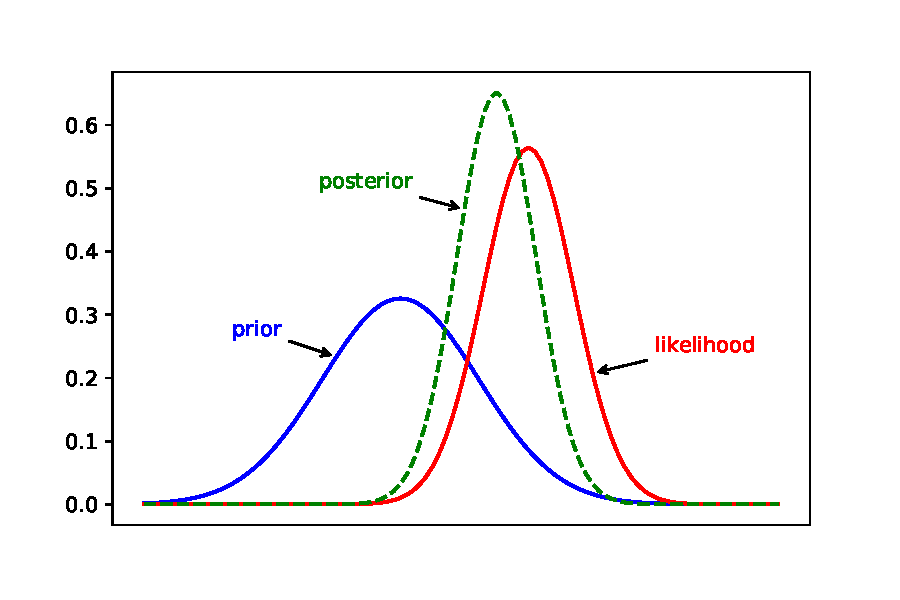
\includegraphics[width=0.45\textwidth]{Imagens/gauss_fusion.pdf}}
	\subfigure[]{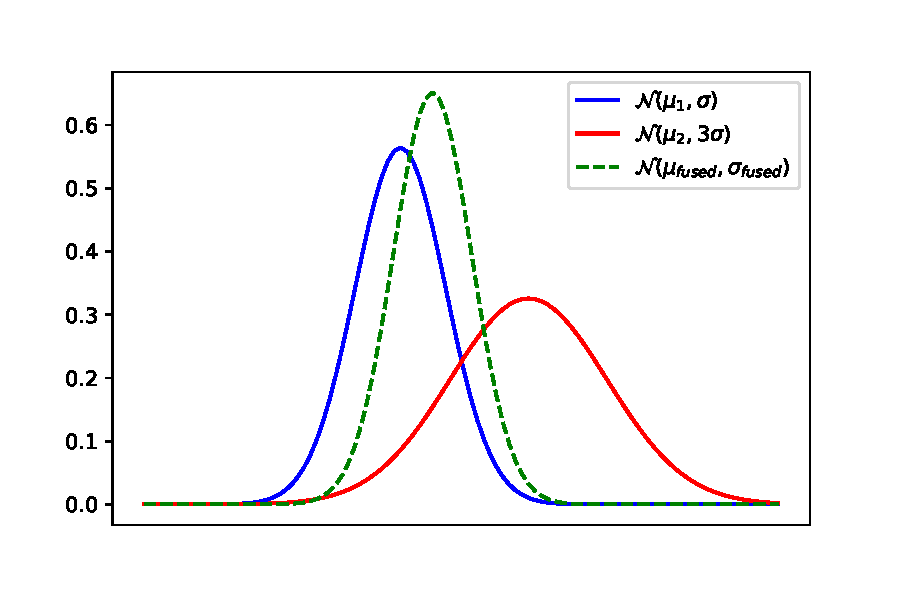
\includegraphics[width=0.45\textwidth]{Imagens/gauss_fusion2.pdf}}
	\caption[\textit{Posterior} PDF obtained by the fusion \textit{prior} and \textit{likelihood}]{\textit{Posterior} PDF obtained by the fusion of \textit{prior} and \textit{likelihood} densities. In (a) the variance of the \textit{likelihood} is smaller than the variance of the \textit{prior}, hence the \textit{posterior} is closer to the \textit{likelihood}. In (b) is the other way around.}
	\label{fig:gauss_fusion}
\end{figure}

\subsection{Kalman Filter}\label{sec:kalman-filter}

The Bayesian recursive solution described by Proposition~\ref{prop:bayes_solution} enables the computation of the optimal estimation of state vector $x_k$. However, its implementation is impossible for practical applications, since it relies on mathematical integrations and as time evolves, the observation sequence grows indefinitely. The sequential algorithm proposed by \citep{Kalman1960} solves that problem adding a restriction in the system assumptions, that is linearity and Gaussianity. 

Consider the Gauss-Markov discrete-time linear system

\begin{align}
x_k &= A_{k-1}x_{k-1} + B_{k-1}u_{k-1} + G_{k-1}w_{k-1}, \label{eq:gm_process}\\
y_k &= C_kx_k+ v_k, \label{eq:gm_obs}
\end{align}

\noindent
where, $\forall k \geq1$, time varying matrices $A_{k-1} \in \mathbb{R}^{n\times n}$,  $B_{k-1} \in \mathbb{R}^{n\times p}$,  $G_{k-1} \in \mathbb{R}^{n\times q}$ and  $C_{k-1} \in \mathbb{R}^{m\times n}$ are known, as well as the input $u_{k-1} \in \mathbb{R}^P$ and output $y_k \in \mathbb{R}^m$ vectors. Process and observation noise vectors, $w_{k-1} \in \mathbb{R}^q$ and $v_{k-1} \in \mathbb{R}^m$ are white, zero-mean and mutually independent, apart from being Gaussian, with known covariance matrices $Q_{k-1}$ and $R_k$, respectively.

Define $\mathcal{N}(x;\bar{x},P^{xx})$ as a multivariate Gaussian PDF on $x$, with mean $\bar{x}$ and covariance $P^{xx}$, given by

\begin{equation}
\mathcal{N}(x;\mu,P^{xx}) \triangleq \frac{1}{(2\pi)^{n/2} \left| P^{xx} \right|^{1/2}}exp\left( -\frac{1}{2}(x-\mu)^T (P^{xx})^{-1}(x-\mu)\right)
\end{equation}

Some identities of multivariate Gaussian probability densities are needed for the next steps and are described in properties ~\ref{prop:joint} and~\ref{prop:marginal}.

\begin{prop} \label{prop:joint}
	If the random variables $x$ and $y$ are Gaussian RVs,
	
	\begin{align}
	\rho(x,y) = \mathcal{N} 
	\left(
	\begin{pmatrix} x \\ y \end{pmatrix};
	\begin{pmatrix} \bar{x} \\ \bar{y} \end{pmatrix},
	\begin{pmatrix} P^{xx} & P^{xy}\\ (P^{xy})^T & P^{yy} \end{pmatrix}
	\right) 
	\end{align}
	
	\noindent
	then, the marginal and conditional PDFs of $x$ and $y$ are given by
	
	\begin{align}
	\rho(x)		&= \mathcal{N}(x; \ \bar{x},\ P^{xx}) \\
	\rho(y) 	&= \mathcal{N}(y; \ \bar{y},\ P^{xy}) \\
	\rho(x|y)  	&= \mathcal{N}(x; \ \bar{x} + P^{xy} (P^{yy})^{-1}(y-\bar{y}),\ P^{xx} - P^{xy} (P^{yy})^{-1} (P^{xy})^T ) \\
	\rho(y|x)  	&= \mathcal{N}(y; \ \bar{y} + (P^{xy})^T (P^{xx})^{-1}(x-\bar{x}),\  P^{yy} - (P^{xy})^T (P^{xx})^{-1} P^{xy})
	\end{align}
	
\end{prop}

\begin{prop} \label{prop:marginal}
	
	If $x$ and $y$ are Gaussian RVs, with PDFs given by
	\begin{align}
	\rho(x) 	&= \mathcal{N}(x;\ \bar{x}, \ P^{xx}), \\
	\rho(y|x) 	&= \mathcal{N}(y;\ Ax, \ P^{yy}),
	\end{align}
	
\noindent
then, the joint and marginal PDFs are defined by
	
	\begin{align}
	\rho(x,y) &= \mathcal{N} 
	\left(
	\begin{pmatrix} x \\ y \end{pmatrix};
	\begin{pmatrix} \bar{x} \\ A\bar{x} \end{pmatrix},
	\begin{pmatrix} P^{xx} & P^{xx}A^T\\ AP^{xx} & AP^{xx}A^T + P^{yy} \end{pmatrix}
	\right), \\
	\rho(y) &= \mathcal{N} (y; \ A\bar{x}, \ AP^{xx}A^T + P^{yy})
	\end{align}
\end{prop}


From the Gauss-Markov assumptions, we can rewrite (\ref{eq:gm_process}) and (\ref{eq:gm_obs}) from a probabilistic perspective, as

\begin{align}
\rho(x_k|x_{k-1}) &= \mathcal{N}(x_k ; \ A_{k-1}\bar{x}_{k-1} + B_{k-1}u_{k-1}, \ Q_k), \label{eq:rho_process}\\
\rho(y_k|x_k) &= \mathcal{N}(y_k; \ C_k\bar{x}_k, \ R_k), \label{eq:rho_obs}
\end{align}

\noindent
where (\ref{eq:rho_process}) is the \textit{transition} density representing the system dynamics and (\ref{eq:rho_obs}) is the \textit{likelihood} density, given by the observation model. 

The Bayesian recursive solution to such system is defined by \textit{forecast} and \textit{data assimilation} steps according to

\begin{align}
\rho(x_{k}|(y_1,...,y_{k-1}) &= \mathcal{N}(x_k; \ \hat{x}_{k|k-1},P^{xx}_{k|k-1}), \label{eq:sol_xk}\\
\rho(x_{k}|(y_1,...,y_{k}) &= \mathcal{N}(x_k; \ \hat{x}_{k|k},P^{xx}_{k|k}) \label{eq:sol_xk1},
\end{align}

\noindent
with the \textit{posterior} density function from a previous step given by

\begin{equation}
\rho(x_{k-1}|(y_1,...,y_{k-1}) = \mathcal{N}(x_{k-1}; \ \hat{x}_{k-1|k-1},P^{xx}_{k-1|k-1}), \label{eq:previous}
\end{equation}

\noindent
where $\hat{x}_{k|k-1}$ and $P^{xx}_{k|k-1}$ are the \textit{forecast} state and covariance estimates, whereas $\hat{x}_{k|k}$ and $P^{xx}_{k|k}$ are the \textit{data assimilation} state and covariance estimates.

Now we combine the \textit{forecast steps} from (\ref{eq:prop_xk1}) and from (\ref{eq:sol_xk}), using the process model from (\ref{eq:rho_process}), the previous estimate from (\ref{eq:previous}) and the identities from property~\ref{prop:marginal}, yielding

\begin{align}
\rho(x_k|(y_1,...,y_{k-1})) &= \int_{\mathbb{R}^n}\rho(x_k|x_{k-1}) \rho(x_{k-1}|y_1,...,y_{k-1})dx_{k-1}, \label{eq:forecast}\\
							&= \mathcal{N}(x_k; \ A_{k-1}\hat{x}_{k-1|k-1} + B_{k-1}u_{k-1}, \ A_{k-1}P^{xx}_{k-1|k-1}A{k-1}^T + G_{k-1}QG_{k-1}^T), \notag
\end{align}

\noindent
that is, the \textit{forecast} state and covariance estimates are computed by

\begin{align}
\hat{x}_{k|k-1} &= A_{k-1}\hat{x}_{k-1|k-1} + B_{k-1}u_{k-1}, \label{eq:forecast_state} \\
P^{xx}_{k|k-1}	&= A_{k-1}P^{xx}_{k-1|k-1}A_{k-1}^T + G_{k-1}QG_{k-1}^T. \label{eq:forecast_cov}
\end{align}

And for the \textit{data assimilation step}, we find the joint density of $y_k$ with the \textit{forecast} estimate from (\ref{eq:forecast}), using property~\ref{prop:joint}

\begin{equation}
\rho(x_k,y_k|(y_1,...,y_{k-1})) = \mathcal{N} 
\left(
\begin{pmatrix} x_k \\ y_k \end{pmatrix}; \
\begin{pmatrix} \hat{x}_{k|k-1} \\ C_k\hat{x}_{k|k-1} \end{pmatrix},
\begin{pmatrix} P^{xx}_{k|k-1} & P^{xx}_{k|k-1}C_k^T\\ C_kP^{xx}_{k|k-1} & C_k P^{xx}_{k|k-1} C_k^T + R_k \end{pmatrix}
\right),	
\end{equation}

\noindent
and the marginal density for $x_k$ is

\begin{equation}
\rho(x_{k}|(y_1,...,y_{k})) = \mathcal{N}(x_k; \ \hat{x}_{k|k-1}+K_k(y_k-C_k\hat{x}_{k|k-1}),P^{xx}_{k|k-1}-P^{xx}_{k|k-1}C_k^T K_k^{-1}P^{xx}_{k|k-1}C_k^T),
\end{equation}
\noindent
that is, the \textit{data assimilation} state and covariance estimates are calculated by

\begin{align}
\hat{x}_{k|k} &= \hat{x}_{k|k-1}+K_k(y_k-C_k\hat{x}_{k|k-1}), \label{eq:assim_state}\\
P^{xx}_{k|k}	&= P^{xx}_{k|k-1}-P^{xx}_{k|k-1}C_k^T K_k^{-1}P^{xx}_{k|k-1}C_k^T. \label{eq:assim_cov}
\end{align}

\noindent
where $K_k \in \mathbb{R}^{n\times m}$ is defined as the Kalman gain and is given by

\begin{equation} \label{eq:kalman_gain}
K_k = P^{xx}_{k|k-1}C_k^T(C_kP^{xx}_{k|k-1}C_k^T + R_k)^{-1}.
\end{equation}

If we define a \textit{forecast} output estimate $\hat{y}_{k|k-1}$, an innovation covariance matrix $P^{yy}_{k|k-1}$ and a cross-covariance matrix $P^{xy}_{k|k-1}$ as 

\begin{align}
\hat{y}_{k|k-1} &\triangleq C_k\hat{x}_{k|k-1}, \\
P^{yy}_{k|k-1} 	&\triangleq E\left[ (y_k-\hat{y}_{k|k-1})(y_k-\hat{y}_{k|k-1})^T \right] = C_kP^{xx}_{k|k-1}C_k^T + R_k , \\
P^{xy}_{k|k-1}	&\triangleq E\left[ (x_k  - \hat{x}_{k|k-1})(y_k-\hat{y}_{k|k-1})^T\right] = P^{xx}_{k|k-1}C_k^T , \\
\end{align}

\noindent
we can simplify \textit{data assimilation} step given by (\ref{eq:assim_state}), (\ref{eq:assim_cov}) and (\ref{eq:kalman_gain}) as

\begin{align}
\hat{x}_{k|k} 	&= \hat{x}_{k|k-1}+K_k(y_k-\hat{y}_{k|k-1}), \label{eq:assim_state2} \\
P^{xx}_{k|k}	&= P^{xx}_{k|k-1}-P^{yy}_{k|k-1} K_k^{-1} (P^{yy}_{k|k-1})^T, \label{eq:assim_cov2} \\
K_k 			&= P^{xy}_{k|k-1}(P^{yy}_{k|k-1})^{-1}. \label{eq:kalman_gain2}
\end{align}


For more details on this derivation, refer to \citep{Sarkka2013}. We summarize the Kalman filter algorithm as below
\begin{algo} \label{alg:KF}Kalman filter (KF) algorithm.
\begin{quote}
\textit{Forecast step}: Using the linear model, calculate the estimated state vector $\hat{x}_{k|k-1}$ and the estimated state covariance $P^{xx}_{k|k-1}$, using (\ref{eq:forecast_state}) and (\ref{eq:forecast_cov}). Calculate Kalman gain $K_k$ by (\ref{eq:kalman_gain}).
\end{quote}
\begin{quote}
\textit{Data assimilation step}: Using the measurement vector $y_k$ and Kalman gain, update estimations from previous step with (\ref{eq:assim_state}) and (\ref{eq:assim_cov}), obtaining estimates $\hat{x}_{k|k}$ and $P^{xx}_{k|k}$.
\end{quote}
\end{algo}

The linear KF is the optimal estimator under both MAP and MMSE criteria, it is unbiased and its cross-covariance will asymptotically achieve the lower bound of the Cram�r-Rao inequality \citep{Teixeira2008}.


\subsection{Unscented Kalman Filter}\label{sec:unscented-kalman-filter}	

For nonlinear systems, the Gaussianity requirement does not hold, even if the uncertainty and initial conditions are Gaussian. Therefore, we can not characterize the posterior PDF only by its first two moments, mean and covariance, and the solution given by proposition~\ref{prop:bayes_solution} are not suited for the estimation problem. In fact, optimal solutions are generally not possible to be obtained by a recursive algorithm.

Adaptations to the Kalman filter have been proposed in the literature. The extended Kalman filter (EKF), for example, linearizes the system around the current state estimates, to achieve approximations using Algorithm~\ref{alg:KF}. A different approach is to approximate the statistics of the posterior PDF, instead of the model. The unscented Kalman filter (UKF) \citep{Julier2004} performs statistical approximations via the unscented transform (UT), based on the Monte Carlo approach.

First, we define a set of samples $\chi \triangleq [\chi_1,...,\chi_{2n}] \in \mathbb{R}^{n\times 2n}$, also referred to as sigma points, to estimate the mean $\bar{x}$ and covariance $\bar{P}^{xx}$ of the random variable being approximated, such that

\begin{align}
\sum_{i=0}^{2n} \gamma_i \chi_i &= \bar{x}, \\
\sum_{i=0}^{2n} \gamma_i \left[ (\chi_i-\bar{x})(\chi_i-\bar{x})^T \right] &= \bar{P}^{xx}, \\
\sum_{i=0}^{2n} \gamma_i &= 1.
\end{align}

\noindent
where $\gamma_{i}$, $\forall i > 1$ are called weights. There are various ways of determining the sigma points, but we choose a simplified version of the original UT proposed by \citep{Julier1997}, which each $\chi_i$ is given by a column of the matrix $\chi = \left[ \chi_1 \ \chi_2 \ \textrm{...} \ \chi_{2n} \right]$ given by


\begin{align}
\chi \triangleq \left[\bar{x} 1_{1\times2n}+\sqrt{n} (\bar{P}^{xx})^{1/2} \quad \ \ \bar{x} 1_{1\times 	2n}-\sqrt{n}(\bar{P}^{xx})^{1/2}\right], \label{eq:sigma_points}
\end{align}

\noindent
with weights

\begin{align}
\gamma = \frac{1}{2n}. \label{eq:weights}
\end{align}

Such simplification has one less tunning degree of freedom to approximate higher order moments of the RV, called scaling factor. We now define the UT algorithm as follows

\begin{algo} \label{alg:UT} Unscented Transform (UT) algorithm
	
\noindent
Consider a nonlinear transformation of two random variables $y$ and $x$

\begin{equation} \label{eq:ut_nonlinear}
	y = f(x,d),
\end{equation}

\noindent where $x$ has mean $\bar{x} \in \mathbb{R}^n$ and covariance matrix $P^{xx} \in R^{n\times n}$ and $d$ is a deterministic vector. First, compute sigma points matrix $\chi$ and its correspondent weights $\gamma$ according to (\ref{eq:sigma_points}) and (\ref{eq:weights}) respectively. Propagate each sigma point $\chi_i$ through the nonlinear transformation given by (\ref{eq:ut_nonlinear}) to find estimated mean $\hat{y}$ and covariance matrix $P^{yy}$ of the RV $y$ and the cross-covariance matrix $P^{xy}$, by
\vspace{-1pt}
\begin{align}
	\Upsilon_i 	&= f(\chi_i,d), \quad \forall i =1,\ ...\ , 2n \label{eq:ut1}\\
	\hat{y} 	&= \sum_{i=0}^{2n} \gamma_i \Upsilon_i, \\
	P^{yy} 	&= \sum_{i=0}^{2n} \gamma_i \left[ (\Upsilon_i-\hat{y})(\Upsilon_i-\hat{y} )^T \right], \\
	P^{xy} 	&= \sum_{i=0}^{2n} \gamma_i \left[ (\Upsilon_i-\hat{y})(\chi_i-\bar{x} )^T \right] \label{eq:ut2}.
\end{align}

For simplicity, we will refer to (\ref{eq:ut1}-\ref{eq:ut2}) as the function $\psi_{UT}$, given by

\begin{equation}
\left[ \hat{y} \ \ P^{yy} \ \ P^{xy}  \right] = \psi_{UT} \left( \bar{x},\ P^{xx}, \ n, \ d, f\right)
\end{equation}

\end{algo}


Based on Algorithm~\ref{alg:UT}, and considering the process and observation models given by (\ref{eq:prob_process}) and (\ref{eq:prob_obs}), the UKF algorithm is as follows

\begin{algo} \label{alg:UKF} Unscented Kalman filter (UKF) algorithm.
	
\noindent
\textit{Forecast step}: Use the UT to calculate the forecast state estimate $\hat{x}_{k|k-1}$ and the respective covariance $P^{xx}_{k|k-1}$ based on last estimation

\begin{equation}
\left[ \hat{x}_{k|k-1} \ \ P^{xx}_{k|k-1} \right] = \psi_{UT} \left( \hat{x}_{k-1|k-1},\ P^{xx}_{k-1|k-1}, \ n, \ d, \ f \right), \label{eq:ukf1}
\end{equation}

\noindent 
where $f$ is given by (\ref{eq:prob_process}) and $d$ by current input data and time instant.

\noindent
Based on forecast state estimate and covariance found in (\ref{eq:ukf1}), compute the forecast observation estimate $\hat{y}_{k|k-1}$, observation vector covariance $P^{yy}_{k|k-1}$ and the cross-covariance between observation and state $P^{xy}_{k|k-1}$, via the UT

\begin{equation}
\left[ \hat{y}_{k|k-1} \ \ P^{yy}_{k|k-1} \ \ P^{xy}_{k|k-1} \right] = \psi_{UT} \left( \hat{x}_{k|k-1},\ P^{xx}_{k|k-1}, \ n, \ d, \ g \right), \label{eq:ukf2}
\end{equation}

\noindent
where $g$ is given by (\ref{eq:prob_obs}) and $d$ by current time instant.

\noindent
\textit{Data assimilation step}: Calculate Kalman gain and current state estimate and covariance at time $k$, same way as in (\ref{eq:assim_state2}-\ref{eq:kalman_gain2}), reproduced for convenience
\begin{align}
K_k					&= P^{xy}_{k|k-1} (P^{yy}_{k|k-1})^{-1}, \\
\hat{x}_{k|k} 		&= \hat{x}_{k|k-1} + K_k(y_k - \hat{y}_{k|k-1}),	 \\
P^{xx}_{k|k}		&= P^{xx}_{k|k-1} - P^{yy}_{k|k-1} K_k^{-1} (P^{yy}_{k|k-1})^T.
\end{align}

\end{algo}


UKF algorithm addresses many of the drawbacks that appear in the EKF implementation, such as the necessity of differentiability, the performance loss due to systems that are poorly approximated by linearization and computational efficiency. Therefore the UKF is the chosen method for the nonlinear system simulated in Chapter~\ref{cap5} and will be further discussed in this section.



	
\section{State Estimation with Aperiodic Sampling} \label{sec:estimation_aperiodic}


The exact solution to the linear discretization problem, defined by (\ref{eq:prob_LTI})-(\ref{eq:wd}) considered digital inputs sampled at the same rate as the observations are taken, producing a sequence of data at time instants $t_k$, $\forall k \in \mathbb{N}$. The nonlinear solution is agnostic to this assumption, since it relies on numerical approximations. Nevertheless, the representation given by (\ref{eq:prob_process3}) and (\ref{eq:prob_obs3}) is constructed using a common time sequence $t_k$, $\forall k \in \mathbb{N}$ for both process and observation models.

However, we are interested in the effects of aperiodic sampling of the observations with data assimilation executed at incorrect time instants, as formulated in Section~\ref{sec:problem_form}. For that, we consider that input signal $u(t)$ is generated by a digital device using an \textit{ideal sampler}, with a regular time interval $T$, that is $u(t)=u(iT)$, for $iT\leq t < (i+1)T$, $\forall i \in \mathbb{N}$. Estimation time instants need to coincide with the regularly spaced time intervals $T$. Measurement instants $t_k$, $\forall k \in \mathbb{N}$ do not match the estimation instants $iT$, $\forall i \in \mathbb{N}$. Additionally, input data $u(iT)$ is available a rate $1/T$ that is $\alpha > 1$ times faster than the expected sampling rate $\lambda$ of the observations. An illustrative example is presented in Figure~\ref{fig:cap4-sampling_example}, where $\alpha=5$, that is the expected time interval for observations $1/\lambda$ is five times higher than regular sampling time interval $T$.

\begin{figure}[!htb]
	\centering
	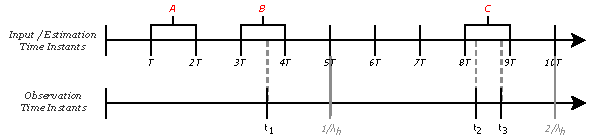
\includegraphics[width=\textwidth]{Imagens/cap4-sampling_example.pdf}
	\caption[Input and observation time instants realization]{Input and estimation time instants labeled as $iT$ and a realization of observation time instants, labeled as $t_k$. Expected time instants for observation is presented in gray, considering that $E[h_k] = \frac{1}{\lambda}$, and $\frac{1}{\lambda} = 5 T$, that is $\alpha=5$.}
	\label{fig:cap4-sampling_example}
\end{figure} 

Between two consecutive estimation time instants, there can be no observation data, illustrated by the red letter \textit{A}, there can be one measurement, red letter \textit{B}, or multiple measurements, shown in the red letter \textit{C}. One example of such application is in target tracking, where inertial sensors that measure process input data such as linear acceleration and angular velocity operate at higher and regular frequencies compared to a network of GPS sensors, that are responsible for the observation model data.

On the next subsections, we present the motivation behind the aperiodic sampling model and discuss how the algorithm is executed for the scenarios when reliable time-stamp information is available, and when it is not part of the data package.

\subsection{Aperiodic Sampling as a Poisson Process}

In Section~\ref{sec:problem_form} we assume the observation time instants $t_k$ occur randomly in time according to a stationary Poisson process. That is, the probability of observing $N(t)=n$ measurements up to and including time $t$ is given by \citep{Papoulis1984}

\begin{equation}
P\left(N(t)=n\right) = e^{-\lambda t}\frac{(\lambda t)^n}{n!}, \label{eq:poissonproc}
\end{equation}

\noindent
where $\lambda$ is called rate or intensity parameter, $t = t_1-t_0$ is the time difference between two points and $N(t)$ is a RV representing the amount of measurements that arrived in the interval given by $t$, as shown in Figure~\ref{fig:poissonproc}. The interarrival time $h_k$, given by the distance between two consecutive arrivals, for the Poisson process has an exponential distribution, with a PDF given by

\begin{equation}
\rho_{h_k}(t) = \lambda e^{-\lambda t}
\end{equation}

\begin{figure}[!htb]
	\centering
	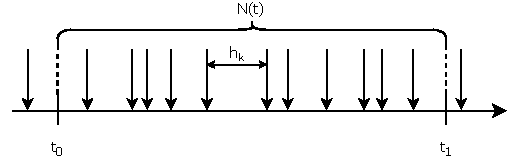
\includegraphics[width=0.6\textwidth]{Imagens/poisson_proc.pdf}
	\caption[Arrivals of a Poisson Process]{Arrivals of a Poisson process between a time interval given by $t=t_1-t_0$. $N(t)$ is the RV representing the discrete amount of arrivals in the time interval and $h_k$ is the distance between two consecutive arrivals.}
	\label{fig:poissonproc}
\end{figure} 

This assumption is proposed by \citep{Micheli2002}, motivated by sensor networks applications. Consider the LTI system described by (\ref{eq:prob_LTI}) and (\ref{eq:prob_LTIobs}). Now assume $N$ sensors measure such system periodically, every $T$ seconds, according to

\begin{equation}
y_i(nT + \xi_i) = Cx(nT + \xi_i) + v(nT + \xi_i), \quad n \in \mathbb{N}, \ i \in \{1,2,...,N\},
\end{equation}

\noindent
where matrix $C$ and measurement noise are already defined in (\ref{eq:prob_LTIobs}) and $\xi_i \in [0,T)$ is referred to as the phase of each sensor, that is the waiting time for the $i$-th sensor to yield a noisy measurement, after time $t=0$. If all phases are different, that is the sensors are not synchronized, and the number of sensors $N$ is high enough, then the amount of measurements arriving in a given interval can be approximated by a Poisson process with rate parameter $\lambda = N/T$. Thus, the random interarrival times or the waiting times between two consecutive measurements can be approximated by an exponential random variable  $h_k \sim \mathcal{E} (\lambda)$, according to Proposition~\ref{prop:poissonproc}.


\begin{propo}\label{prop:poissonproc} Let the phases of all sensors $\{\xi_i\}_{i=1}^N$ be i.i.d uniform random variables in the interval $[0,N/\lambda]$, with $\lambda \in \mathbb{R}$ and $N \in \mathbb{N}$. Now define $h_N = \textrm{min}(\xi_1,\xi_2,...\xi_N)$ as the first interarrival time, occurring in  $[0,N/\lambda]$. Then, the RV $h_N$ converges in distribution to an exponential RV, that is
	
\begin{equation}
h_N \xrightarrow[]{D} \mathcal{E}(\lambda),
\end{equation}
	
\noindent
where $\xrightarrow[]{D}$ means \textit{converges in distribution}, as $N\rightarrow \infty$.
	
\end{propo}

\begin{proof} The distribution of $h_N$ is studied by the so called extreme value theory \citep{Leadbetter1983}. To compute it, we consider its cumulative distribution function (CDF), given by	
	
\begin{align}
\rho_{h_N} \left( \textrm{min}_i(\xi_i) \leq \right) &= 1 - \rho\left( \textrm{min}_i(\xi_i) \geq t \right), \\
 &= 1 -  \rho\left( \xi_1 \geq t, \ \xi_2 \geq t,..., \ \xi_N \geq t \right),\\
 &= 1 - \prod_{i=1}^N \rho(\xi_i \geq t), \\
 &= 1 - \prod_{i=1}^N \left[ 1- \rho(\xi_i \geq t) \right], \\
 &= 1 - \left[ 1- \rho(\xi_i \geq t) \right]^N.
\end{align}

continuar expli�ao com base em

https://danieltakeshi.github.io/2016/09/25/the-expectation-of-the-minimum-of-iid-uniform-random-variables/

\end{proof}







%\subsection{Input Irregular Sampling}
%
%Em caso de amostragem irregular tamb�m na entrada, um esquem�tico dos instantes de estima��o, amostragem e entrada pode ser observado na Fig.~\ref{fig:esquema2}
%
%\begin{figure}[!htb]
%	\centering
%	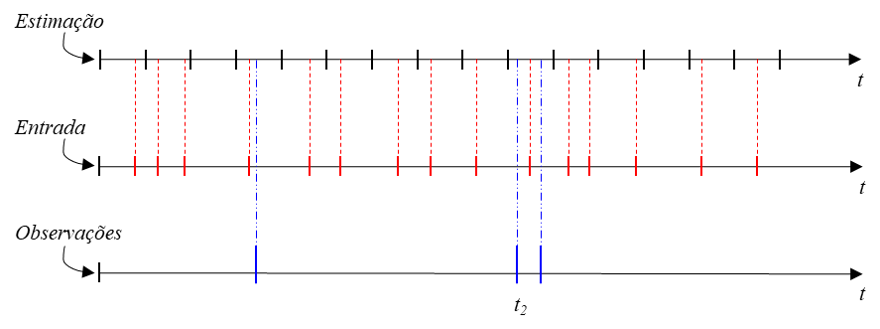
\includegraphics[scale=0.65]{Imagens/esquema3}
%	\caption[Exemplos de instantes de amostragem de estima��o]{Exemplos de instantes de amostragem de estima��o(1), da entrada (2) e das observa��es (3). Os instantes m�ltiplos de $\lambda$, igual ao intervalo m�dio de amostragem das observa��es s�o apresentados em cinza escuro, para refer�ncia.}
%	\label{fig:esquema2}
%\end{figure} 
%
%Para atrasos de transmiss�o:
%
%\begin{figure}[!htb]
%	\centering
%	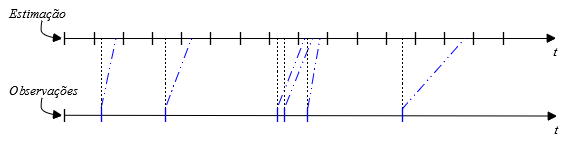
\includegraphics[scale=0.65]{Imagens/esquema4}
%	\caption[Exemplos de instantes de amostragem de estima��o com atraso de tempo]{Exemplos de instantes de amostragem de estima��o(1), da entrada (2) e das observa��es (3). Os instantes m�ltiplos de $\lambda$, igual ao intervalo m�dio de amostragem das observa��es s�o apresentados em cinza escuro, para refer�ncia.}
%	\label{fig:esquema3}
%\end{figure} 
%
%Nas pr�ximas subse��es � apresentado como os algoritmos de estima��o tratam os cen�rios \textbf{A}, \textbf{B} e \textbf{C} para os casos em que o carimbo de tempo est� e n�o est� dispon�vel.
%

\subsection{With Timestamp}\label{sec:carimbo}

If the estimator knows the exact time $t_k$ that measurements were taken in a global timescale, \textit{data assimilation} steps can be performed at the correct time instants. For that, the process model discretization given by (\ref{eq:prob_process3}) is performed considering variable time intervals $\delta t_j^*$, yielding

\begin{equation}\label{eq:disc_carimbo}
x(t^*_j)=f_\textrm{d}(x(t^*_{j-1}),u(t^*_{j-1}),w(t^*_{j-1}),t^*_{j-1}),
\end{equation}

\noindent
where $t^*_j$, $\forall j \in \mathbb{N}$ represents the estimation time sequence and is given by $t^*_j= t^*_{j-1} + \delta t^*_j$, with $t^*_0=0$. The variable time interval $\delta t^*_j$ is calculated according the schematic presented by Figure~\ref{fig:cap4-online_estimator}.

\begin{figure}[!htb]
	\centering
	\begin{adjustbox}{width=0.65\textwidth,height=\textheight,keepaspectratio}
		
		\begin{tikzpicture}[node distance=2cm, font = \scriptsize]
		
		\node(start)[startstop][text width=2.8cm,align=center]{\textbf{Start} \\ $t^*_0=0$; \\ $i=j=k=1$; \\};
		
		\node (dec1) [decision, below of=start,yshift=-0.5cm] {Signal Received};
		
		\node (pro1) [process, below right of=dec1, yshift=-0.9cm, xshift=0.25cm][text width=2.8cm,align=center]{Calculate \\ $\delta t^*_{j} = iT - t^*_{j-1}$ \\ $t^*_{j} = t^*_{j-1} + \delta t^*_{j}$};
		
		\node (pro12) [process, below of=pro1][text width=2.8cm,align=center, yshift=0.5cm]{Forecast Step};
		
		\node (pro2) [process, below left of=dec1,  yshift=-0.9cm, xshift=-0.25cm][text width=2.8cm,align=center]{Calculate \\ $\delta t^*_{j} = t_k - t^*_{j-1}$ \\ $t^*_{j} = t^*_{j-1} + \delta t^*_{j}$};
		
		\node (pro22) [process, below of=pro2][text width=2.8cm,align=center, yshift=0.5cm]{Forecast Step, using ZOH};
		
		\node (pro23) [process, below of=pro22][text width=2.8cm,align=center, yshift=0.7cm]{Data Assimilation \\ Step};
		
		\node (pro3) [startstop, below of = pro23][text width=2.8cm,align=center, xshift=1.8cm]{Estimate in $t^*_{j}$};
		
		\draw [arrow] (start) -- node[pos=0.5](h){} (dec1);
		\draw [arrow] (dec1) -| node[text width=2.8cm,align=center,anchor=west,xshift=-1cm] {Iput \\ Signal} (pro1);
		\draw [arrow] (dec1) -| node[text width=2.8cm,align=center,anchor=east,xshift=0.8cm] {Observation\\ Signal} (pro2);
		\draw [arrow] (pro1) -- (pro12);
		\draw [arrow] (pro2) -- (pro22);
		\draw [arrow] (pro22) -- (pro23);
		\draw [arrow] (pro12) -- node[text width=2.8cm,align=center,anchor=south,xshift=0.8cm, yshift=-1cm] {$i=i+1$} (pro3);
		\draw [arrow] (pro23) -- node[text width=2.8cm,align=center,anchor=east,xshift=0.6cm] {$k=k+1$}(pro3);
		\draw [arrow] (pro3) --+(-4cm,0) |- node[text width=2.8cm,align=center,anchor=south,xshift=1cm] {$j=j+1$}(h);
		\end{tikzpicture}
	\end{adjustbox}
	
	\caption[Illustrative schematic of the \textit{online} estimator, with time-stamp]{Illustrative schematic of the \textit{online} estimator, with time-stamp. indices $i$, $j$ e $k$ represent the input, estimation and observation signal counters, respectively.}
	\label{fig:cap4-online_estimator}
\end{figure}	


Each value $\delta t^*_j$ corresponds to the time interval between the last instant $t^*_{j-1}$ in which a signal was received, whether it transmitted input or observation data, and the next time interval $t^*_{j}$ in which a new signal arrives. A zero order holder (ZOH) is used for input signals, considering last available information. 

For the simulation carried out in Section~\ref{cap5}, time intervals $\delta t^*_j$ are calculated by uniting all arrival times for input and observation in a single vector, in an orderly fashion. The subtraction of consecutive time instants yields the time intervals sequence $\delta t^*_j$, $\forall j \geq 1$. 

Since there are two signal types, input and observation, there are four possible cases for the estimator: input followed by another input; input followed by an observation; observation followed by an input; and observation followed by another observation. In Figure~\ref{fig:cap4-sampling_example}, all of them are represented. During the interval \textit{A}, there are only input signals, so time interval is $T$ and only \textit{forecast} is performed. In the interval represented by \textit{B}, we have to first execute complete \textit{forecast} and \textit{data assimilation} steps between input and observation, from $3T$ until $t_1$, using $\delta t^*_4 =t_1-3T$. Next, between an observation and an input signal, a ZOH is used for a \textit{forecast} step between $t_1$ and $4T$. In other words, it is considered that the input remained constant between $3T$ and $4T$. When more than one observation arrive between two input signals, as in \textit{C}, full \textit{forecast} and \textit{data assimilation} are performed as many times needed before one last \textit{forecast} between the last observation and the next input signal.

For the \textit{online} estimator, the differential equations are numerically integrated as input or measurement signals arrive. In these instants, the corresponding time interval $\delta t^*_j$ is calculated. If the current signal transmits input data, only the \textit{forecast} step is executed. If it is observation data being received, both \textit{forecast} and \textit{data assimilation} steps are performed, considering a ZOH for the input data. 


\subsection{Without Timestamp}

On the other hand, in case there is no information about time-stamp, process model (\ref{eq:prob_process}) is discretized according to


\begin{equation}\label{eq:disc_semcarimbo}
x_n=f^*_\textrm{d}(x_{n-1},u_{n-1},w_{n-1},n),
\end{equation}

\noindent
where $f^*_\textrm{d}(\cdot)$ represents the time-invariant discrete-tmie mode and $n=nT$, $\forall n \in \mathbb{N}$.

Since the estimator is not aware of the measurement time instant, \textit{data assimilation} is always performed as the next input signal arrives, in a time instant multiple of $T$. In such cases, there are only two possible scenarios. One, in which there are no information between two consecutive input signal arrivals, represented by the letter \textit{A} in Figure~\ref{fig:cap4-sampling_example}, when only \textit{forecast} step is performed. If there is observation, full \textit{forecast} and \textit{data assimilation} steps are performed, considering the time interval $T$. In case illustrated by the letter \textit{B}, measurement taken at time $t_1$ will be assimilated in time instant $4T$. When there are multiple measurements between two input signals, the oldest ones are discarded, as in letter \textit{C}, for which the measurement taken at $t_2$ is discarded and the one taken at $t_3$ is assimilated at the instant $9T$.


\section{Performance Metrics} \label{sec:metrics}

In order to assess the performance degradation introduced by assimilating data at incorrect time instants, we need to define certain performance metrics for comparison. The algorithms described in Sections~\ref{sec:unscented-kalman-filter} and~\ref{sec:kalman-filter} estimate both the current state, $\hat{x}_{k|k}$ and its covariance matrix $\hat{P}^{xx}_{k|k}$. For the linear case, the \textit{posterior} conditional PDF 
$\rho(x_{k}|(y_1,...,y_{k})$ is Gaussian, according to (\ref{eq:sol_xk1}), so it is fully characterized by its first two moments. Thus, if the filter is consistent, the following conditions shall be met \citep{Bar-Shalom2001}

\begin{align}
E\left[x_k - \hat{x}_{k|k}\right] &\triangleq E[\tilde{x}_{k|k}] = 0, \label{eq:consistency1} \\
E\left[(x_k - \hat{x}_{k|k})(x_k - \hat{x}_{k|k})^T\right] &\triangleq E[\tilde{x}_{k|k}\tilde{x}_{k|k}^t] = P^{xx}_{k|k}, \label{eq:consistency2}
\end{align}

\noindent
where $\tilde{x}_{k|k}$ is the estimation error at time instant $k$. Condition (\ref{eq:consistency1}) is called \textit{unbiasedness} requirement, whereas (\ref{eq:consistency1}) refers to \textit{covariance matching}. For the nonlinear case, these conditions cannot be fully met, since the \textit{posterior} PDF is an approximation of a Gaussian density. Thus, the closer they are met, the more consistent are the filter estimates.
%
In this study we will use metrics that measure both consistency conditions. According to Bar-Shalom, in order to test them, the consistency criteria metrics for state estimation must certify: that state estimate errors are zero mean and compatible with the estimated state covariance; that innovations are also zero mean and compatible with their respective covariances; and that innovations are white. We will adopt two tests proposed by him that attests all conditions simultaneously, that is the normalized (state) estimation error squared (NEES) and normalized innovation squared (NIS) tests. We first defined NEES and NIS as


\begin{align}
NEES_k &\triangleq  \tilde{x}_{k|k}^T(P^{xx}_{k|k})^{-1}\tilde{x}_{k|k}, \label{eq:nees} \\
NIS_k &\triangleq  \eta_{k|k-1}^T(P^{yy}_{k|k-1})^{-1}\eta_{k|k-1}, \label{eq:nis}.
\end{align}

Under the linear and Gaussian assumption, we formulate a hypothesis test, under which the null hypothesis $H_0$, that the filter is consistent, requires that both NEES and NIS follow chi-squared distributions, with $n_x$ and $n_y$ degrees of freedom, respectively, and $n_x$ is the dimension of the state vector, whereas $n_y$ is the dimension of the observation vector. The expected value of a RV that is chi-squared distributed is equal to its degrees of freedom quantity, that is $E[NEES_k] = n_x, \ \forall k > 1$ and  $E[NIS_k] = n_y, \ \forall k > 1$. 

We adopt single-run tests, thus for every estimation, we test the acceptance of $H_0$, that is if both NEES and NIS at time instants $k$ are within a certain interval, considering the accepted region as 

\begin{align}
P \left\{ NEES_k \in [r_1,r_2] | H_0 \right\} &= 1 - \alpha, \label{eq:nees_h0} \\
P \left\{ NIS_k \in [r_1,r_2] | H_0 \right\} &= 1 - \alpha, \label{eq:nis_h0}
\end{align}

\noindent
where $\alpha$ is the significance level and interval $[r_1,r_2]$ is given by the chi-square distribution degrees of freedom and $\alpha$. For instance, considering a system with a state vector of size 4 and observation vector of size 2, and a significance level of $\alpha=5\%$, the acceptance intervals for NEES and NIS are respectively given by

\begin{align}
\left[\chi^2_2(0.025),\ \chi^2_2(0.975)\right] &= [0.051, \ 7.38], \label{eq:nees_interval} \\
\left[\chi^2_4(0.025),\ \chi^2_4(0.975)\right] &= [0.484, \ 11.1], \label{eq:nis_interval}
\end{align}

\noindent
which means that, if the filter is consistent, in $95\%$ of the estimates, NEES and NIS value should fall under their correspondent intervals. Figure~\ref{fig:chi2plots} shows both $\chi^2_2$ and $\chi^2_4$ PDFs, with the $95\%$ acceptance region.

\begin{figure}[!htb]
	\centering
	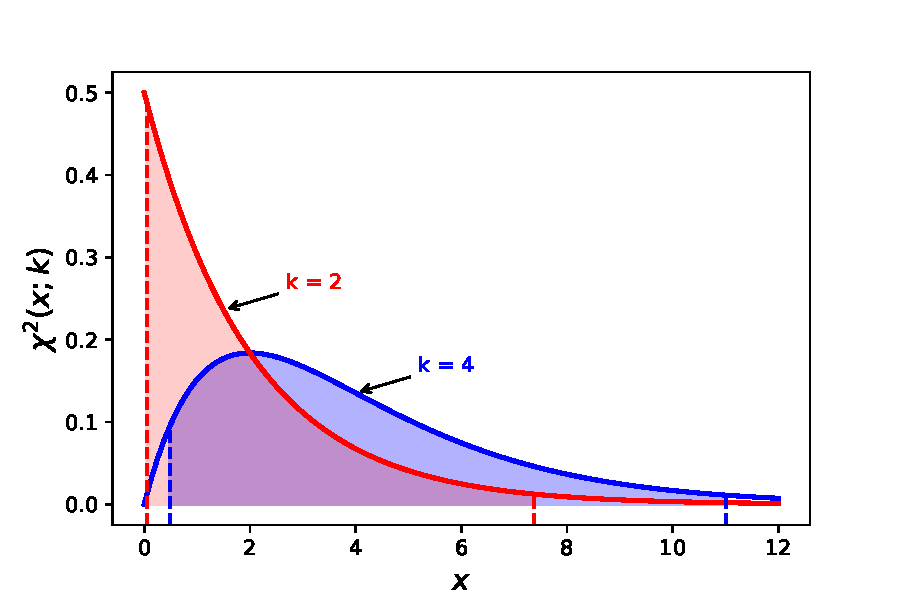
\includegraphics[width=0.75\textwidth]{Imagens/Esquemas/chi2.pdf}
	\caption[$\chi^2$ PDFs and acceptance regions]{$\chi^2$ PDFs for 2 (red) and 4 (blue) degrees of freedom. The vertical dashed lines represent the acceptance interval limits, for $\alpha=5 \% $, and the shaded area is the corresponding acceptance regions.}
	\label{fig:chi2plots}
\end{figure} 


Additionally, since we are using simulated systems, the root mean square error (RMSE) of the system states will also be calculated as an accuracy performance index, given by


\begin{equation}\label{eq:rmse}
RMSE = \frac{ \sum_{i=1}^N \sqrt{(\hat{x}_{k|k}-x_{k})^2}}{N}
\end{equation}

\noindent
where $x_k$ is the true state vector and $N$ is the amount of estimates.


\clearpage